\documentclass[xcolor ={table,usenames,dvipsnames}]{beamer}
\usepackage[italian]{babel}
\usepackage{listings}
\usepackage{txfonts}
\PassOptionsToPackage{dvipsnames}{xcolor}
\title{Multivariate Analysis and Statistical Learning \\PC Algorithm's implementation}

\author{Authors: Alex Foglia, Tommaso Puccetti}
\institute{Universit\`a  degli Studi di Firenze}
\date{21/12/2018}
%\usepackage{sansmathaccent}
\usetheme{Berlin} 
\useinnertheme{rounded}
\useoutertheme{miniframes} 
\setbeamercovered{dynamic}
 
\theoremstyle{definition}
\newtheorem{definizione}{Definizione}

\begin{document}
	
	\begin{frame}
		\maketitle
	\end{frame}

	\begin{frame}
		\frametitle{Theorical references (1)}
		\begin{itemize}
			\item Bayesian Networks can be rappresented as a \textbf{directed acyclic graph (DAG)}
			\item "acyclic" means that there are no paths starting from a node $v$ that ends with $v$ itself, $\forall v \in G$
			
		\end{itemize}
	\end{frame}

	\begin{frame}
		\frametitle{Theorical references (2)}
		Let $G = (V,E)$ be a DAG relative to a finite set  $X = \{X_v \forall v \in V\}$ of casual variables, then:
		$$
		\forall u,v \in V \;non\;adjacent\;| v \in nd(u) \Rightarrow u \Perp v | nd(u) - v
		$$
	Where $nd(u)$ is the set of \textbf{non-descendant} n of n, that are all those nodes $u'$ for which there is no path from $u$ to $u'$. \\
	\end{frame}

	\begin{frame}
		\frametitle{PC-Algorithm}
		Given a set of variables with a joint Gaussian probability distribution, it is possible to learn the DAG closer to the sample through the use of  \textbf{PC-Algorithm}. \\
		It is composed of two sub-functions that solve two different problems:
		\begin{enumerate}
			\item The construction of the skeleton (or \textbf{Moral Graph})
			\item The construction of the DAG from a given skeleton
		\end{enumerate}
	\end{frame}

	\begin{frame}
		\frametitle{Pseudocode: skeleton generation}
		\begin{figure}[h!]
			\centering
			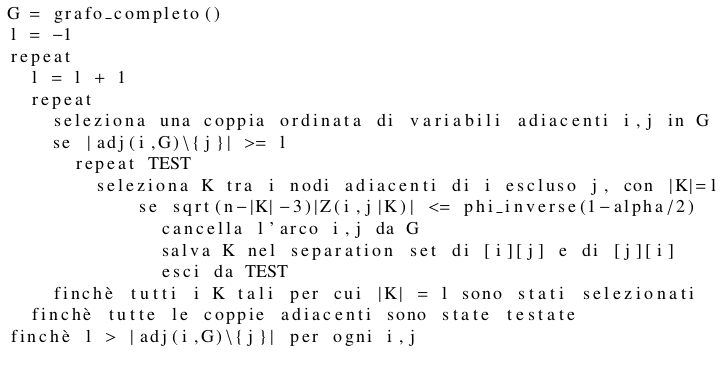
\includegraphics[scale=0.53]{img/pcalg.PNG}
			\label{Interfacce di un CS}
		\end{figure}
	\end{frame}

%	\begin{frame}
%		\frametitle{Pseudocodice: costruzione del DAG}
%		\begin{figure}[h!]
%			\centering
%			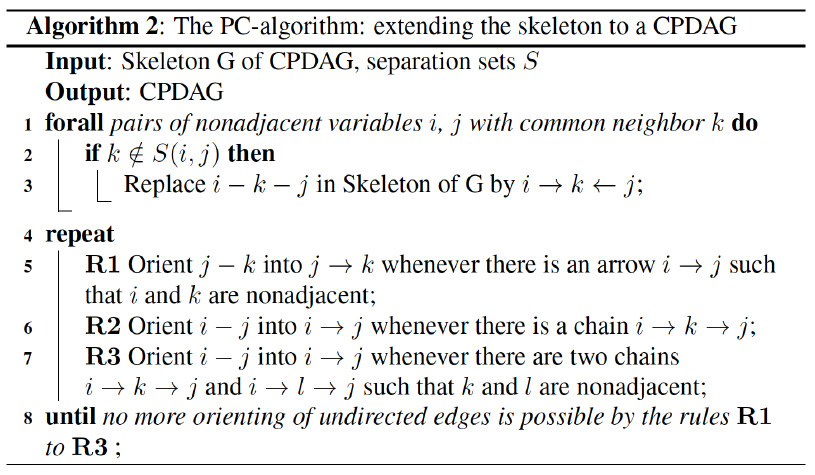
\includegraphics[scale=0.5]{img/pcalg2.PNG}
%			\label{Interfacce di un CS}
%		\end{figure}
%	\end{frame}

%	\begin{frame}
%		\frametitle{Skeleton generation: get\_skeleton()}
%		\begin{enumerate}
%			\item Calculate the \textit{variance/covariance} matrix using the \textit{\textbf{cov()}} function on the dataset.
%			\item Calls the \textit{\textbf{PC\_algorithm()}} wich implements the main core of skeleton generation.
%			\item The function can be called passing the \textit{correlation} matrix of the dataset. By default this input parameter is setted to "None".
%			\item Calculate the \textit{sigma inverse} using the function \textit{\textbf{pinv()}} on variance/covariance matrix
%		\end{enumerate}
%	\end{frame}
	
	
	\begin{frame}
		\frametitle{PC-Algorithm for the skeleton: implementation (1)}
		\begin{itemize}
			\item If the corr\_matrix parameter is setted to "None" then call the \textit{\textbf{tocor()}} function that returns the \textit{correlation} matrix from sigma matrix.
			\item Initialize the \textit{adjacency matrix} G of the \textit{complete graph} with all the elments equals to 1, and set the diagonal elements to 0.
			\item Instantiate the function \textit{\textbf{adj()}} that takes a node x and return the neighbour of x.
		\end{itemize}
		INSERIRE CODICE CORR
	\end{frame}

	\begin{frame}
		\frametitle{Skeleton generation: implementation (2)}
		\begin{enumerate}
			\item Set  counter $l$ to zero.
			\item Iterating all the elements of the matrix, append in the act\_ind list all of the couples x,y of nodes that has an edge in common.
			\item Taken a couple x,y in act\_ind, create the set of neighbor relative to x using the \textit{\textbf{adj()}} function.
			\item Calculate the set of all possible combinations of nodes from the neighbor's set, with lenght equal to l.
			\item Do the \textbf{independence test} for x,y data K, for all K in neighbor set:
			\begin{itemize}
				\item if $pvalue < alpha$ then delete the edge x,y and y,x from the adjacency matrix.
			\end{itemize}
			\item Repeat for every elements of the adjacency matrix.      
		\end{enumerate}
	\end{frame}

	\begin{frame}
		\frametitle{Skeleton generation: implementation (3)}
	\end{frame}

	
\end{document}